\documentclass[11pt]{article}
\usepackage[review]{acl}
\usepackage{times}
\usepackage{latexsym}
\usepackage[T1]{fontenc}
\usepackage[utf8]{inputenc}
\usepackage{microtype}
\usepackage{booktabs}
\usepackage{graphicx}
\newcommand{\nDisc}{46,846}
\newcommand{\wDisc}{439}
\newcommand{\hetSDisc}{57}
\newcommand{\nRep}{4,684}
\newcommand{\wRep}{46}
\newcommand{\hetSRep}{57}
\newcommand{\nConf}{13,945}
\newcommand{\wConf}{171}
\newcommand{\hetSConf}{62}
\newcommand{\agrDisc}{0.064}
\newcommand{\agrDiscCI}{[0.045, 0.079]}
\newcommand{\othDisc}{0.018}
\newcommand{\othDiscCI}{[0.010, 0.026]}
\newcommand{\nulDisc}{[$-$0.008, 0.008]}
\newcommand{\pairsDisc}{50,690}
\newcommand{\agrRep}{0.114}
\newcommand{\agrRepCI}{[0.068, 0.168]}
\newcommand{\othRep}{$-$0.022}
\newcommand{\othRepCI}{[$-$0.055, 0.013]}
\newcommand{\nulRep}{[$-$0.070, 0.094]}
\newcommand{\pairsRep}{411}
\newcommand{\agrNoPrint}{0.063}
\newcommand{\agrPrint}{0.062}
\newcommand{\agrPrintCI}{[0.040, 0.083]}
\newcommand{\printAlone}{0.010}
\newcommand{\printAloneCI}{[$-$0.001, 0.022]}
\newcommand{\sSub}{0.014}
\newcommand{\sSubP}{0.014}
\newcommand{\sdGap}{0.69}
\newcommand{\sdBg}{2.2}
\newcommand{\placeboT}{0.033}
\newcommand{\placeboTp}{.041}
\newcommand{\fuClauseFive}{0.016}
\newcommand{\fuClauseFiveCI}{[0.009, 0.022]}
\newcommand{\fuClauseFiveHeld}{0.014}
\newcommand{\fuClauseFiveHeldCI}{[0.003, 0.025]}
\newcommand{\fuClauseStrict}{0.015}
\newcommand{\fuClauseStrictCI}{[0.009, 0.022]}
\newcommand{\fuClauseStrictHeld}{0.013}
\newcommand{\fuClauseStrictHeldCI}{[0.002, 0.024]}
\newcommand{\fuCtx}{0.031}
\newcommand{\fuCtxCI}{[0.020, 0.042]}
\newcommand{\fuCtxHeld}{0.034}
\newcommand{\fuCtxHeldCI}{[0.019, 0.050]}
\newcommand{\fuNc}{$-$0.008}
\newcommand{\fuNcCI}{[$-$0.023, 0.007]}
\newcommand{\fuNcHeld}{$-$0.007}
\newcommand{\fuNcHeldCI}{[$-$0.031, 0.016]}
\newcommand{\fuCtxLow}{0.013}
\newcommand{\fuCtxLowCI}{[0.003, 0.023]}
\newcommand{\fuCtxLowHeld}{0.012}
\newcommand{\fuCtxLowHeldCI}{[$-$0.004, 0.028]}


\title{The Space Between Words: Word Predictability Leaves a Small Trace in Handwritten Spacing}
\author{Anonymous submission}
\date{}

\begin{document}
\maketitle

\begin{abstract}
Keystrokes and speech timing reveal how language is planned, but a handwritten page records only where the ink landed. We ask whether the space between handwritten words still carries linguistic information. Using 656 writers copying English text in the IAM database, with analysis decisions fixed in advance and a held-out set of writers opened once, we relate inter-word gaps to language-model surprisal and parse structure after controlling for letter shapes, word length, frequency and layout. A word that is one standard deviation more surprising is preceded by a gap \(0.036\) core heights wider in the held-out writers, about 5\% of a within-line standard deviation. The effect is small, is roughly halved when only lowercase words are considered, and is weak for any individual writer. Two syntactic measures were positive in discovery but did not reach significance in the held-out set. Separately, writers copying the same sentence agree on where to leave more space, beyond what the word pair alone predicts. That agreement is not explained by the spacing of the printed text they copied, but in discovery it comes almost entirely from one group of texts, and it could not be tested on held-out writers.
\end{abstract}

\section{Introduction}
Language production leaves measurable traces. Speakers lengthen less predictable words \citep{demberg2012}, typists slow down at uncertain letters \citep{crump2019} and at prosodic boundaries \citep{fuchs2016}, and keystroke timing can even help a shallow parser \citep{plank2016}. Handwriting research finds similar effects in pen timing, including longer intervals at syllable boundaries during copying \citep{kandel2006}.

These signals all need a time-stamped recording. Most handwriting ever produced has none: it survives as a static image. We ask whether the \emph{spatial} layout of offline handwriting carries any linguistic signal. Specifically, when people copy text by hand, is the gap between two words wider when the next word is less predictable or when a larger syntactic boundary falls between them?

The answer matters beyond psycholinguistics. Handwriting generators such as VATr \citep{pippi2023}, TS-GAN \citep{davis2020} and Emuru \citep{pippi2025} treat spacing as style or as a by-product of the letters. If spacing also depends on the language, then evaluating or modelling it as a purely visual property leaves part of the signal out.

We make three contributions: (1) a pre-specified measurement of how word surprisal and syntactic structure relate to handwritten gaps, confirmed on writers held out until the analysis was frozen; (2) a model-free test of whether different writers leave similar gaps at the same point of the same sentence; and (3) a direct test of the main confound specific to copying: writers imitating the spacing of the printed text.

We report the limits of these findings as prominently as the findings. The effects are small, and only the surprisal effect survives in held-out writers.

\section{Data and Measures}
\paragraph{Data.} We use IAM \citep{marti2002iam}, in which writers copied passages of the LOB corpus \citep{johansson1978lob} printed at the top of a form. A \emph{prompt} is one such passage; a \emph{boundary} is two adjacent words on one handwritten line, both containing a letter or digit, in a line whose segmentation IAM marks as correct. Clitics are excluded, and because IAM tokenises punctuation separately, gaps next to a separate comma or period are not measured.

\paragraph{Outcome.} Gap is the horizontal distance between the ink of the two words, in units of the line's median core (x-) height, measured at full 300\,dpi resolution. The within-line SD of the gap is \sdGap{} core heights.

\paragraph{Linguistic predictors.} Each is standardised on the Discovery set. \emph{Surprisal} is the GPT-2-large \citep{radford2019} negative log-probability, in bits, of the right word given all preceding text of the form \citep{hale2001,smith2013}. \emph{Tree distance} is the path length between the two words in a Stanza \citep{qi2020} constituency parse, a measure of boundary strength. \emph{Clause onset} marks a right word that begins an embedded clause (labels S, SBAR, SBARQ, SINV or SQ; see Section~\ref{sec:followups} for the label set the plan named).

\paragraph{Controls.} Character counts of both words (total, uppercase, digit, ascender, descender), the identity of the left word's last and right word's first character, log frequency of both words, position in the line and remaining width. We remove controls from both outcome and predictors with models cross-fitted by prompt and fitted on Discovery only, then centre within line. This is the partialling-out form of an OLS with line fixed effects. Standard errors are clustered by writer.

\section{Study Design}
We wrote the analysis plan before linking any gap to a linguistic variable. Writers were divided into three disjoint sets: Discovery (\wDisc{} writers, \nDisc{} boundaries, including lines by writers outside any official IAM split), Replication (\wRep{} writers, \nRep{}) and Confirmation (\wConf{} writers, \nConf{}: the official validation-2 and test writers). Confirmation gaps were not computed until the code was frozen, and the analysis was run once. The three predictors form one family, Holm-corrected \citep{holm1979}. The plan and all deviations will be released with the paper.

Before analysing real data we validated the estimator on gaps shuffled within line, which destroys any linguistic signal. Planting known effects of \(+0.05\) on surprisal and \(+0.03\) on tree distance moved the estimates by \(+0.050\) and \(+0.030\) respectively, with no effect on the other predictors.

\section{Results}
\paragraph{Linguistic predictors.} Table~\ref{tab:main} and Figure~\ref{fig:effects} give the joint model. In Discovery all three predictors are positive and significant. In Replication, a small set, all are positive with similar magnitudes, but only clause onset excludes zero. In Confirmation, surprisal is positive and significant, while tree distance and clause onset are not. Our pre-registered rule required a Discovery effect to replicate with a confidence interval above zero. Strictly applied, only clause onset met it in Replication, and only surprisal then held in Confirmation. No predictor passed every stage.

\begin{table}[t]
\centering\scriptsize
\setlength{\tabcolsep}{3pt}\begin{tabular}{@{}lccc@{}}
\toprule
 & Surprisal & Tree distance & Clause onset \\
\midrule
Discovery & 0.026 & 0.021 & 0.017 \\
\quad 95\% CI & [0.013, 0.038] & [0.013, 0.029] & [0.009, 0.025] \\
\quad Holm $p$ & $<$.001 & $<$.001 & $<$.001 \\[2pt]
Replication & 0.022 & 0.021 & 0.026 \\
\quad 95\% CI & [$-$0.004, 0.049] & [$-$0.001, 0.042] & [0.006, 0.045] \\
\quad Holm $p$ & .126 & .126 & .029 \\[2pt]
Confirmation & 0.036 & 0.014 & 0.009 \\
\quad 95\% CI & [0.015, 0.057] & [$-$0.002, 0.030] & [$-$0.004, 0.022] \\
\quad Holm $p$ & .003 & .182 & .188 \\[2pt]
Pooled & 0.027 & 0.020 & 0.016 \\
\quad 95\% CI & [0.017, 0.038] & [0.013, 0.026] & [0.009, 0.022] \\
\bottomrule
\end{tabular}

\caption{Added gap (core heights) per SD of each predictor, joint model. Pooled is inverse-variance across the three writer sets and includes Discovery, so it is descriptive.}
\label{tab:main}
\end{table}

\begin{figure}[t]
\centering
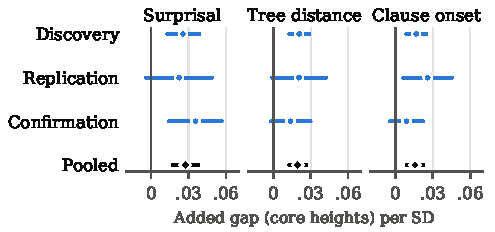
\includegraphics[width=\columnwidth]{fig_effects.pdf}
\caption{Estimates with 95\% CIs, clustered by writer. Circles are individual writer sets; diamonds are the pooled estimates.}
\label{fig:effects}
\end{figure}

\paragraph{Size.} The pooled surprisal effect is 0.027 core heights per SD, 4\% of the within-line SD. Together the three predictors explain 0.2\%--0.4\% of within-line residual gap variance. The surprisal slope is positive for only \hetSDisc\%--\hetSConf\% of writers with enough data, so this is a population regularity, not a reliable property of an individual's page.

\paragraph{Robustness.} Table~\ref{tab:robust} reports the pre-stated checks, pooled. Surprisal is stable under word-class tags, flexible controls, clipping and a different language model, Pythia-1B \citep{biderman2023}. It halves when both words are lowercase. Part of the effect therefore depends on boundaries involving names, capitals or digits. Clause onset nearly vanishes once word-class tags are added: it is largely a property of words such as \emph{that} and \emph{to}. Tree distance survives tags.

\begin{table}[t]
\centering\footnotesize
\setlength{\tabcolsep}{3pt}\begin{tabular}{@{}lccc@{}}
\toprule
Specification & Surprisal & Tree dist. & Clause onset \\
\midrule
Primary & \textbf{0.027} & \textbf{0.020} & \textbf{0.016} \\
Lowercase words only & \textbf{0.013} & \textbf{0.012} & \textbf{0.015} \\
+ LOB tags & \textbf{0.027} & \textbf{0.027} & {0.005} \\
GBM controls & \textbf{0.027} & \textbf{0.016} & \textbf{0.013} \\
Gap clipped 1--99\% & \textbf{0.026} & \textbf{0.019} & \textbf{0.016} \\
Pythia surprisal & \textbf{0.026} & \textbf{0.019} & \textbf{0.016} \\
\bottomrule
\end{tabular}

\caption{Pooled estimates under each pre-stated check. Bold: 95\% CI excludes zero. Pooled values include Discovery.}
\label{tab:robust}
\end{table}

A placebo outcome, the mean background intensity around the two words, should be unrelated to language. Surprisal and clause onset were. Tree distance had a small Discovery effect (\placeboT{} grey levels per SD, Holm \(p=\placeboTp\); within-line SD \sdBg) that did not recur in Replication or Confirmation. We cannot rule out a small measurement artefact in tree distance.

\paragraph{Agreement between writers.} After controls, we correlate the residual gaps of different writers at the same boundary of the same prompt. In Discovery the correlation is \agrDisc{} \agrDiscCI{} over \pairsDisc{} writer pairs. The same word pair in a \emph{different} prompt correlates only \othDisc{} \othDiscCI, and shuffling boundaries within a form gives a null band of \nulDisc. In Replication the values are \agrRep{} \agrRepCI{} and \othRep{} \othRepCI, against a null band of \nulRep, on only \pairsRep{} pairs. Spacing thus depends on the specific sentence, not just the words at the boundary.

This result has a sharp limit. Nine prompts from one IAM text group (g06), each copied by many writers, contribute 85\% of Discovery pairs and all correlate positively (0.05 to 0.14). Across the other 53 prompts the correlation is 0.019, the same as the different-prompt reference. Agreement is therefore not established outside that group in Discovery. The Replication result (13 prompts from a different text group, f, two writers each) is the only independent support. No prompt in Confirmation was copied by two writers, or shared with another set, so agreement could not be tested there.

\paragraph{Could writers be copying the printed spacing?} The IAM prompts are typeset with full justification, so printed spaces vary. We measured them on the scanned forms (median scan-to-scan SD 0.7\,px where a prompt was scanned repeatedly), for prompts in the forms A--H. The printed gap did not significantly predict the handwritten gap (pooled \printAlone{} \printAloneCI). Controlling for it changed the agreement only from \agrNoPrint{} to \agrPrint{} \agrPrintCI, and left the linguistic coefficients essentially unchanged (surprisal \sSub{} to \sSubP). On this restricted set, which drops repeated word pairs, surprisal is smaller than in the full data. This analysis was added after Confirmation and is exploratory.

\paragraph{Follow-up checks.}\label{sec:followups} Both checks were specified in writing before being computed, but after all writer sets had been seen, so they are exploratory. Estimates pool the three sets, and in parentheses Replication and Confirmation alone. First, is the surprisal effect about context, or about the word? We added each word's context-free surprisal (its GPT-2-large probability after only the start-of-text token). With this held fixed, in-context surprisal is \fuCtx{} \fuCtxCI{} (\fuCtxHeld{} \fuCtxHeldCI), and context-free surprisal itself is \fuNc{} \fuNcCI. The effect is thus carried by predictability in context. For lowercase-only boundaries, however, in-context surprisal is \fuCtxLow{} \fuCtxLowCI, below our 0.02 size threshold, and its interval includes zero without Discovery (\fuCtxLowHeld{} \fuCtxLowHeldCI). Second, our code labelled clause onsets with SINV and SQ in addition to the S, SBAR and SBARQ named in the plan. Using the plan's three labels changes the pooled estimate from \fuClauseFive{} to \fuClauseStrict{} \fuClauseStrictCI; the conclusions do not change.

\section{Discussion and Limitations}
Word predictability leaves a real but very small trace in handwritten spacing, of a size that a reader would not notice on a single line. The result extends production effects known from speech and typing to a static spatial record. Its practical value for reading linguistic structure off a page is, at this size, low.

\textbf{Copying is not composing.} IAM writers copied printed text, so the results concern copying, in which writers may break text into chunks when they look back at the source. \citet{olive2002} found similar process activation in copying and composing, but composition may behave differently. \textbf{A gap is not a pause.} Without pen timing we can only infer a link to processing time. \textbf{Selection and scope.} We analyse lines with correct IAM segmentation, English only, and 1960s text assessed by modern models. \textbf{Agreement is concentrated.} In Discovery the between-writer result comes almost entirely from one text group, and it lacks a held-out test. \textbf{Generators are untested.} We did not measure whether handwriting generators reproduce this effect; such a test needs thousands of generated lines to detect an effect of this size, and remains future work.

\section{Conclusion}
The spacing of handwritten words is not purely visual. Less predictable words are preceded by slightly wider gaps, in writers held out from every analysis decision, and in some texts different writers partly agree on where to leave space in a given sentence. Both effects are small, the agreement lacks a held-out test, and syntactic measures did not hold up in held-out writers.

\bibliography{references}
\end{document}
